\documentclass{article}

\author{Jonathan Michel}

\title{RSolve Manual}

\usepackage{float}
\usepackage{graphicx}
\usepackage{amsmath}
\usepackage{amsfonts}
\usepackage{lmodern}
\usepackage{wrapfig}
\usepackage{hyperref}
\hypersetup{colorlinks=false}
\usepackage{cite}

\begin{document}

\maketitle

\tableofcontents

\section{Introduction}

This manual describes RSolve, a suite of software to create networks and
evaluate their electrical resistances. Networks are lattice-based, and can
be hierarchical, in the sense that, when a network is constructed, each of
its bonds can be replaced by a finer-scale network. This process can, in
principle, be repeated \emph{ad infinitum}. At each length scale, disorder
can be added in two ways: by randomly removing a subset of connections in
the network, and by adding position disorder to the vertices of the network.

Once a netwok is created, it can be reported in three distinct ways: as a
planar line graph, as an SVG file, and as an extruded surface stored in an STL
file. The last two options were designed to allow
the creation of physical specimens for experimental work. STL files can also
be imported by software packages that can be used to create FEM meshes to
allow finite element simulation of current flow. This method differs from
that used by the program \texttt{rsolve}, described below.

This project originated with graduate work at Georgia Tech in the lab of
Professor Peter Yunker. Professor Yunker supplied the original idea for the
project and supported the development of the initial version of this software.
I have also benefitted from discussions with Henry Murphy, whose testing of
the software's capabilities highlighted numerous opportunities for improvement.
This software has benefitted from the open source software packages SuiteSparse,
by Timothal Alden Davis, and Triangle, by Jonathan Richard Shewchuk.

\section{Installation}

This software is written mostly in standard C++. It depends on the C-language
library Triangle, by Jonathan Richard Shewchuk, as well as Shewchuk's
geometric predicates library. These need not be installed by the user; rather,
lightly modified versions of the source code for these software packages are
included with the RSolve source code. The RSolve library also requires
SuiteSparse, a library for solving large linear systems involing sparse
matrices, such as those that are typically encountered when studying networks of
resistors. SuiteSparse, in turn, requires efficient BLAS and LAPACK libraries. I
have personally linked SuiteSparse against the Intel MKL implementations of
these libraries. Choosing efficient BLAS and LAPACK libraries is 
\emph{extremely} important to ensure good performance from this software.
Certain SuiteSparse capabilities require OpenMP to be installed as well, and
some SuiteSparse components can be further expedited by CUDA.

Apart from the specialized dependencies mentioned above, this software requires
a modern C and C++ compiler, as well as GNU Make. Once all dependencies are
installed, building the library should be as simple as typing ``\texttt{make}''.
This should build a subdirectory called \texttt{lib}, as well as the
executables \texttt{hnet\_maker} and \texttt{rsolve}.

\section{Constructing Networks with \texttt{hnet\_maker}}

\subsection{Overview}

The program \texttt{hnet\_maker} operates in two modes: interactive and
automated. In the interactive mode, the program prompts the user for each
stage of the network creation process. In the automated mode, an input
file is passed to the program using the syntax \texttt{-j file\_name}.
Information is parsed from the job file and used to automatically generate
one more more networks. While the interactive mode may be useful for tinkering
while designing a parameter sweep, the automated mode is likely much more
useful for production runs. In the next subsection, the network creation process
is described in detail. In the following subsections, specific explanations of 
the interactive and automated modes are provided.

\subsection{Network Construction Process}

Whatever the mode of operation, network creation is organized into levels.
At each level, a network structure is specified in terms of a lattice and
a scale factor that sets the lattice spacing. Lattices are built row-by-row
within a set of prescribed Cartesian bounds. Lattice information is read from
.lat files, which specify the locations of vertices and the displacements from
vertices to neighbors to which those vertices are connected by a bond. Four such
files are provided by default tri.lat, hcmb.lat, kag.lat, and square.lat, which
produce triangular, honeycomb, Kagome, and square lattices, respectively. If the
program will be run from a different directory, it can be useful to set the
\texttt{LAT\_DIR} system variable to the directory in which the software is
installed, so that fully qualified paths do not have to be entered.

Disorder can be applied to networks in two ways: vertices of the network can be
randomly displaced according to a Gaussian distribution, and connections between
vertices can be removed, such that the of proportion of retained vertices is 
$p$, with $p \in (0, 1]$. Dilution of bonds can be carried out either by 
ensuring all vertices belong to a single connected component, or by a purely 
random process. Purely random dilution can be specified by the \texttt{-d} flag.

After the first network structure has been applied, an arbitrary number of 
additional levels of structure can be specified. Note that levels should
be specified in order of \emph{increasing} length scale. At each level, the
user must specify the width of the bonds. For all but the smallest length
scale, the user \emph{must} specify a width greater than zero. Also note that,
for good results, lattices across scales should generally have structures and
lattice constants such that they are commensurate - that is, large-scale
vertices coincide with small-scale vertices in a regular pattern. The 
large-scale network structure may also be disordered by displacing vertices
and removing bonds.

If position disorder is added to large-scale vertices in a hierarchical
network, the user may specify that a grain-based approach should be used.
This means that as much of each large-scale edge as possible will be filled with
a small-scale lattice with a specified structure. At boundaries between
grains constructed in this manner, edges will be formed connecting vertices
within some cutoff distance such that no two edges intersect. If two
prospective edges would intersect, the shorter of the two edges will be chosen.

Once all levels of strcuture are specified, network creation proceeds in
the opposite order of that in which levels are specified. For hierarchical
network creation, once a network is generated at a given length scale, each
bond is given a non-zero width to generate an envelope. The network one level
below this network in the hierarchy is then created, and only bonds falling
within the large-scale envelope are kept. When small-scale bonds are diluted in
a hierarchical network, they are removed in such a way that the large-scale bond
topology is preserved.

If vertices at any length scale are displaced to create site disorder, there
will, in general, be no clearly defined top and bottom edges of the network.
This will make it challenging to define well-posed boundary conditions to
simulate the resistance of a network. To address this issue, the user may
specify that the network should be prepared for grips. If this option is
selected, the user must specify lower and upper y coordinates such that
bonds protruding below or above these bounds will be truncated at the
prescribed heights.

\subsection{Alternate Output Forms}

By default, once a network has been constructed, it is reported in a file format
that first specifies the number of vertices and edges, then lists all vertices,
and finally specifies edges as pairs of integer indices into the list of
vertices. While this offers a concise description of the network, I have found
it useful to report networks by specifying networks by enumerating edges only.
In this more verbose format, each edge is specified by three lines. The first
two lines give the Cartesian components of the endpoints of the edge, and
the third line is blank. This output mode can be selected using the 
``\texttt{-v}'' switch. Note that this verbose format is appropriate only
for quick visualization -- the program \texttt{rsolve} expects networks to
be reported in the concise format.

In addition to specifying networks as planar line graphs, i.e. a set of vertices, and edges connecting those vertices, there are two modes to enable the
fabrication of physical samples. SVG files can be created by passing the
``\texttt{-s}'' switch. If this mode is used, the network at the smallest scale 
should have bonds of non-zero width. This mode is intended to allow the creation
of samples that can be made with a laser cutter or drag knife plotter. In this
mode, the user must specify additional information about tabs to append to
the top and bottom of the network. Tab outlines have four components:
outward-curving quarter ellipse arcs, rounded corners, vertically aligned
parallel edges, and horizontally oriented top and bottom edges. The user
must specify the width and height of elliptical arcs, the radius of curvature
of corners and the heights of the final top and bottom tabs.

STL files may also be generated, and can be used for 3D printing and as
a precursor to FEM mesh construction. In this case, networks at the smallest
scale also must have a non-zero width. Networks are extruded out of the plane
by a user-specified height. The resulting surface is triangulated and written
to a binary STL file. 

\subsection{Auxilliary Information}

In addition to the network itself, information can be stored about the
network at the largest length scale, the degree to which small-scale bonds
are aligned with the large-scale bonds in which they lie, and the polygonal
tiling into which the large-scale envelope is partitioned in preparation for
selecting small-scale edges. Reporting of the alignment is requested with
the ``\texttt{-a}'' switch, and reporting of the large-scale polygonal
tiling is requested with the ``\texttt{-p}'' switch.

\subsection{Interactive Mode}

In the interactive mode, the required information is requested one field at
a time through a series of command line prompts. The expected answer may be
one or more numbers, a string literal, or, in the case of yes/no questions,
either ``\texttt{y}'' of ``\texttt{n}''. While perhaps useful as a preliminary
means of exploring different options, this method is not very efficient when
preparing for parameter sweeps. One could create a shell script to automate
interaction, but a more elegant alternative is described below.

\subsection{Automated Mode}

In the automated mode, all necessary information for network construction
is specified in a special script file format. This format is organized into
hierarchcially arranged \emph{elements}, each of which may have zero or more
child elements. An element begins with a name and an opening left curly brace,
and ends with a closing right curly brace. Apart from child elements, elements
may also have \emph{attributes}. These are specified using the syntax
\texttt{element\_name = "value"}. A value may either be a single entity or
multiple entities delimited by spaces. After a name-value pair has been 
specified, it should be separated from any successive member of an element by a
comma. In addition to the specification of elements and attributes, the user may
also include blank lines and comment lines. A comment line is distinguished by
the property that its first non-whitespace character is a pound sign. These
characteristics collectively define a serialization scheme I have named
ISLE (Input Serialization LanguagE) \footnote{It may seem odd to design one's
own serialization language, but I couldn't find one that suited my criteria.}.
By convention, I give these files the extension .isle.

In the context of \texttt{hnet\_maker}, the outermost element of an ISLE file
should be ``\texttt{hnet\_job}''. This element must have as children one or
more elements of type ``\texttt{layer}''. The outer \texttt{hnet\_job} element
should have at least the attributes \texttt{bounds} and \texttt{output\_name}.
The value of the \texttt{bounds} attrtibute should be a list of four numbers,
giving the minimum $x$ and $y$ coordinates and maximum $x$ and $y$ coordinates
of the bounding box containing the network. The output name should be a string,
to which additional information and a file extension will be appended to
create the file name for exporting a newly created network.

The \texttt{hnet\_job} element supports numerous optional attributes. If
site disorder is added to vertices on any length scale, it will likely be
desirable to specify heights at which the network should be truncated to create
clean top and bottom boundary conditions. This can be accomplished by
setting the attibute \texttt{add\_grips} to ``true''. One must also set the
attribute \texttt{grip\_heights} in this case, with a value of a top and bottom
truncation height, separated by whitespace.

Multiple realizations for each unique combination of network construction
parameters may also be requested. This is accomplished by setting the
attribute \texttt{realizations} to an integer greater than $1$.

If a range of bond occupations is specified at a given construction stage
(see below), multiple different combinations of network parameters will be
created. In this case, numerical labels will be appended to the base output
name to indicate the bond occupation. By default, three decimal digits will
be used. This value can be changed by setting the attribute
\texttt{report\_digits}.

If a network is to be deluted, by default, dilution begins with the
construction of a random minimum spanning tree. If completely random bond
removal is preferred, this can be accomplished by setting the attribute
\texttt{connected} to ``false''.

If the user wishes to ensure adjacent vertices along the top and bottom of
the network are joined by bonds, this can be accomplished by setting the
parameter \texttt{connect\_top\_bottom} to ``true''. This feature may be
deprecated in the future.

As noted above, various sorts of auxiliary information apart from the final
network can be reported. In the automated mode, these options can be activated
by setting the following output file name patterns to a non-empty string:

\begin{itemize}
\item \texttt{alignment\_file}: A record of the degree of alignment of small scale bonds with the large-scale bonds within which they are contained
\item \texttt{poly\_file}: The file containing the polygonal tiles into which
the top-level envelope is partitioned
\item \texttt{skeleton\_file}: A file containing the ``skeleton'' of the 
top-level envelope, before a non-zero width is imparted to each bond
\item \texttt{top\_file}: A file containing the top-level envelope used to
judge whether small-scale bonds should be included
\end{itemize}

Each \texttt{layer} element within the \texttt{hnet\_job} parent element
should have at least the following properties:

\begin{itemize}
\item \texttt{lattice\_file}: The name of a lattice description file from which
to read information about network geometry and topology
\item \texttt{scale}: A scale factor to set the lattice constant at a given
length scale
\item \texttt{width}: The width of each bond in the network
\item \texttt{bond\_occupation}: The fraction of bonds to retain. This
quantity should either be a single number between zero and one, inclusive, or
a minimum value, maximum value, and step size.
\end{itemize}
If a range of bond occupations is specified, a job will be created for each
bond occupation in this range. If a range of bond occupations is specified
for multiple levels, then the total number of networks created will be the
product of the numbers of distinct bond occupations at each length scale.

The \texttt{layer} element also has a number of optional attributes. If the
user wishes to apply Gaussian random noise the vertex positions, this can
be specified with the field \texttt{displacement}, which gives the standard
deviation of this noise. For any level of structure below one for which
position disorder is added, the corresponding \texttt{layer} element can
specify that grain-based construction should be used by setting the
attribute \texttt{grain\_based} to true. In this case, the parameter
\texttt{stitch\_cutoff}, giving the greatest length of a bond stitching two
grains, should also be specified.

To make the above concepts more concrete, two sample job files are provided
below. The first demonstrates the creation of a small hierarchical network
to be reported to a file as a planar line graph.

\begin{figure}[!htb]
\framebox[\textwidth]{
\begin{minipage}[c]{\textwidth}
\texttt{
\\hnet\_job \{
\newline
\\\hspace*{4ex}output\_name = "tri\_tri\_2\_2\_1\_p1",
\\\hspace*{4ex}bounds = "0 0 2 2",
\newline
\\\hspace*{4ex}\#The structure at the small length scale
\\\hspace*{4ex}layer \{
\\\hspace*{8ex}lattice\_file= "tri.lat",
\\\hspace*{8ex}scale = ".1",
\\\hspace*{8ex}width = "0",
\\\hspace*{8ex}bond\_occupation = "1",
\\\hspace*{4ex}\}
\newline
\\\hspace*{4ex}\#The structure at the large length scale
\\\hspace*{4ex}layer \{
\\\hspace*{8ex}lattice\_file= "tri.lat",
\\\hspace*{8ex}scale = "1",
\\\hspace*{8ex}width = ".2",
\\\hspace*{8ex}bond\_occupation = "1",
\\\hspace*{4ex}\}
\\\}
}
\end{minipage}
}
\caption{This ISLE file generates a hierarhical triangular lattice in which
large-scale bonds are 10 times the length of small-scale bonds.}
\label{fig:simple_ht_isle_file}
\end{figure}

%\begin{wrapfigure}[11]{r}{.5\textwidth}
\begin{figure}[h]
\centering
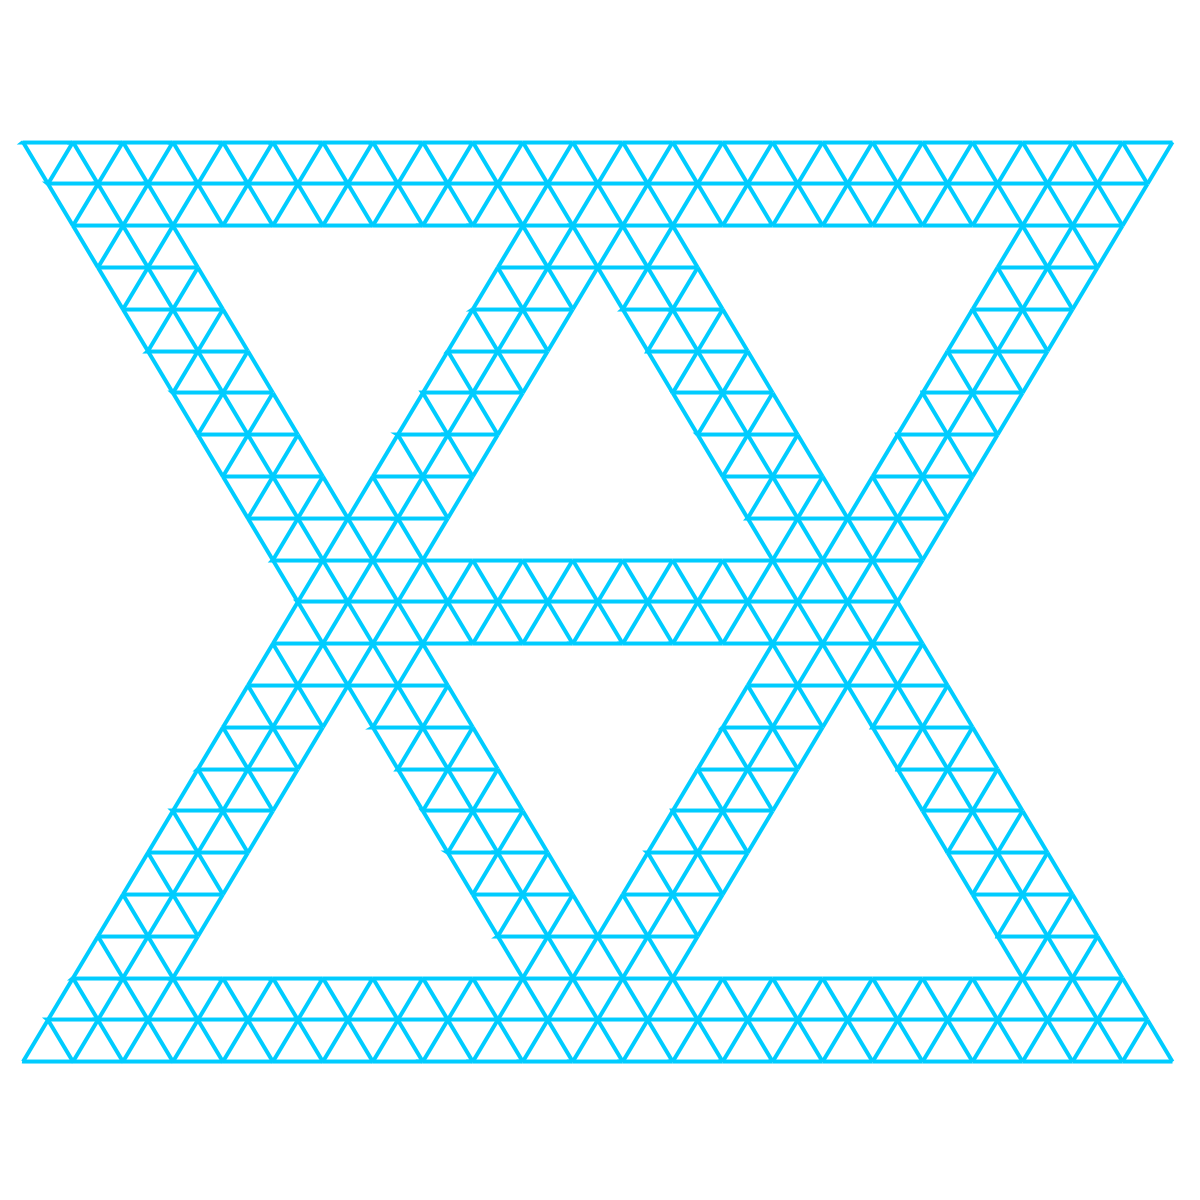
\includegraphics[width=.5\textwidth]{figures/tri_tri_2_2_1_p1.png}
\caption{A small, hierarchical triangular lattice created by the script in
Figure \ref{fig:simple_ht_isle_file}.}
\end{figure}
%\end{wrapfigure}

The ISLE file in Figure ~\ref{fig:svg_stl_ht_isle_file} demonstrates the
creation of SVG and STL files. The attributes for both types of output are
included. One can choose which sort of output is actually created from the
command line, by supplying either the ``\texttt{-s}'' switch for SVG output or
the ``\texttt{-e}'' switch for output as an extruded surface in the STL format.
Unneeded attributes will simply be ignored, such that a single job file can
do double duty. The results of these two usage modes are displayed in Figure
\ref{fig:svg_stl_comparison}.

\begin{figure}[H]
\framebox[\textwidth]{
\begin{minipage}[c]{\textwidth}
\texttt{
\\hnet\_job \{
\newline
\\\hspace*{4ex}output\_name = "tri\_tri\_2\_2\_1\_p1",
\\\hspace*{4ex}bounds = "0 0 2 2",
\\\hspace*{4ex}extrusion\_height = "0.02",
\\\hspace*{4ex}taper\_width = ".25",
\\\hspace*{4ex}taper\_height = ".5",
\\\hspace*{4ex}corner\_radius = ".1",
\\\hspace*{4ex}tab\_height = ".5",
\newline
\\\hspace*{4ex}\#The structure at the small length scale
\\\hspace*{4ex}layer \{
\\\hspace*{8ex}lattice\_file= "tri.lat",
\\\hspace*{8ex}scale = ".1",
\\\hspace*{8ex}width = "0.02",
\\\hspace*{8ex}bond\_occupation = "1",
\\\hspace*{4ex}\}
\newline
\\\hspace*{4ex}\#The structure at the large length scale
\\\hspace*{4ex}layer \{
\\\hspace*{8ex}lattice\_file= "tri.lat",
\\\hspace*{8ex}scale = "1",
\\\hspace*{8ex}width = ".2",
\\\hspace*{8ex}bond\_occupation = "1",
\\\hspace*{4ex}\}
\\\}
}
\end{minipage}
}
\caption{This ISLE file generates a hierarhical triangular lattice in which
large-scale bonds are 10 times the length of small-scale bonds, but differs
from the example above in that small-scale bonds have non-zero width, and
attributes are specified to support SVG and STL file creation.}
\label{fig:svg_stl_ht_isle_file}
\end{figure}

\begin{figure}
\centering
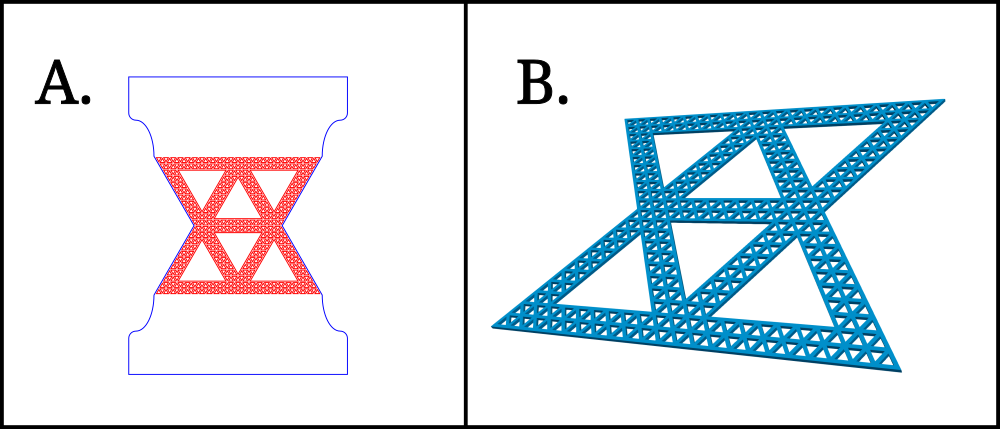
\includegraphics[width=\textwidth]{figures/svg_stl_comparison.png}
\caption{The results of running \texttt{hnet\_maker} with the job file in
Figure \ref{fig:svg_stl_ht_isle_file} are shown. Panel
\textbf{A} shows the output produced by the ``\texttt{-s}'' switch, and panel
\textbf{B} shows the output produced by the ``\texttt{-e}'' switch.}
\label{fig:svg_stl_comparison}
\end{figure}

\section{Solving for Potentials and Resistances}

Interaction with \texttt{rsolve} is fairly simple. The user can either supply
the name of a network description file at the command line using the switch
\texttt{-f}, or run the program in interactive mode, in which case the program
will prompt the user for a file. If the user wishes for the potential to be
written to a file, this can be indicated by the \texttt{-p} flag, which takes
as an argument the name of the file to which the potential of each node should
be written. In interactive mode, triggered by running the program with no
input, the user is asked if a potential file is desired, and upon answering
in the affirmative, the user is asked for the name of this file.

The simulation carried out by \texttt{rsolve} is one in which unit potential
difference is applied to the network. At the moment, the program is designed
with the assumption that each resistor is of the same resistance. In the future,
this assumption may be relaxed to allow for the study of heterogeneous
resistor networks.

To compute the resistance of a network, the potential is required. Any node in
the network not at either the top or bottom is required to have no net current
passing into or out of it. Nodes at the top and bottom are required to have
prescribed electric potentials. These conditions collectively can be used to
define a matrix $\mathbf{A}$. Let the vector 
$\vec{\varphi} \in \mathbb{R}^{1 \times N}$ be a list of potentials of all
nodes, where $N$ is the number of nodes in the network. If a node is on
the interior of the network, the steady state condition dictates that
the total current flowing in or out of the node is zero. The current flowing
to node $i$ from node $j$ is 

\begin{equation}
\phi_{ij} = \frac{\phi_j - \phi_i}{R_{ij}},
\end{equation}
where $R_{ij}$ denotes the the resistance of the resistor connecting these
two nodes. Let $nn(i)$ denote the set of all nodes $j$ connected to node $i$
by a resistor. If node $i$ is an interor node, the $i$th row of $\mathbf{A}$ is
then defined by 

\begin{equation}
a_{ij} =
\begin{cases}
\frac{1}{R_{ij}}, & j \in nn(i)\\
-\sum_{k \in nn(i)} \frac{1}{R_{ik}}, & j = i\\
0, & \text{otherwise},
\end{cases}
\end{equation}
where $a_{ij}$ denotes the $j$th component of the $i$th row of $\mathbf{A}$. If
the node $i$ is on the top or bottom of the network, the corresponding row of 
$\mathbf{A}$ has a simpler form:

\begin{equation}
a_{ij} = \delta_{ij}, 
\end{equation}
where $\delta$ denotes the Kronecker delta function.

The potential is then obtained by solving the equation

\begin{equation}
\label{eq:potential_equation}
\mathbf{A} \vec{\varphi} = \vec{b},
\end{equation}
where $\vec{b} \in \mathbb{R}^{1 \times N}$ is defined by

\begin{equation}
b_{i} = \begin{cases}
1, & i \text{\hspace{1ex} is a top vertex}\\
0, & \text{otherwise}.
\end{cases}
\end{equation}
Equation ~\eqref{eq:potential_equation} is solved by \texttt{rsolve} using
the sparse QR decomposition package of the SuiteSparse library.

With the solution for the potential in hand, the resistance is computed by
dividing the potential difference across the network by the current flowing
through the network. Denoting the set of top vertices by $\mathcal{T}$,
the current flowing into the top vertices of the network, $I_{top}$, is given
by

\begin{equation}
I_{top} = \sum_{i \in \mathcal{T}} \sum_{j \in nn(i)} \frac{\phi_j - \phi_i}{R_{ij}}.
\end{equation}
As the simulation assumes a unit potential difference between the top and
bottom of the network, the network resistance, $R_{net}$, is computed as

\begin{equation}
R_{net} = \frac{1}{I_{total}}.
\end{equation}

\nocite{*}
\bibliographystyle{plain}
\bibliography{rsolve_manual}{}

\end{document}
